\section{Experiment 2 - The effect of different boundary conditions when applying mean curvature flow on signed distance fields.}
In this experiment we would like to examine how different boundary conditions influence the end result of applying mean curvature flow to a signed distance field. When deriving the mean curvature flow we run into boundary issues as we need the values surrounding a grid cell to compute its value. One way to deal with this is to pad the grid with an extra 'layer' such that when we compute the values inside the grid, we can use these 'extra' values to avoid out of bound errors. However, which values should we pad with? In \autoref{boundaryConditions} we have depicted a signed distance field and three boundary conditions we will look at in turn.
\begin{figure}[H]
	\centering
	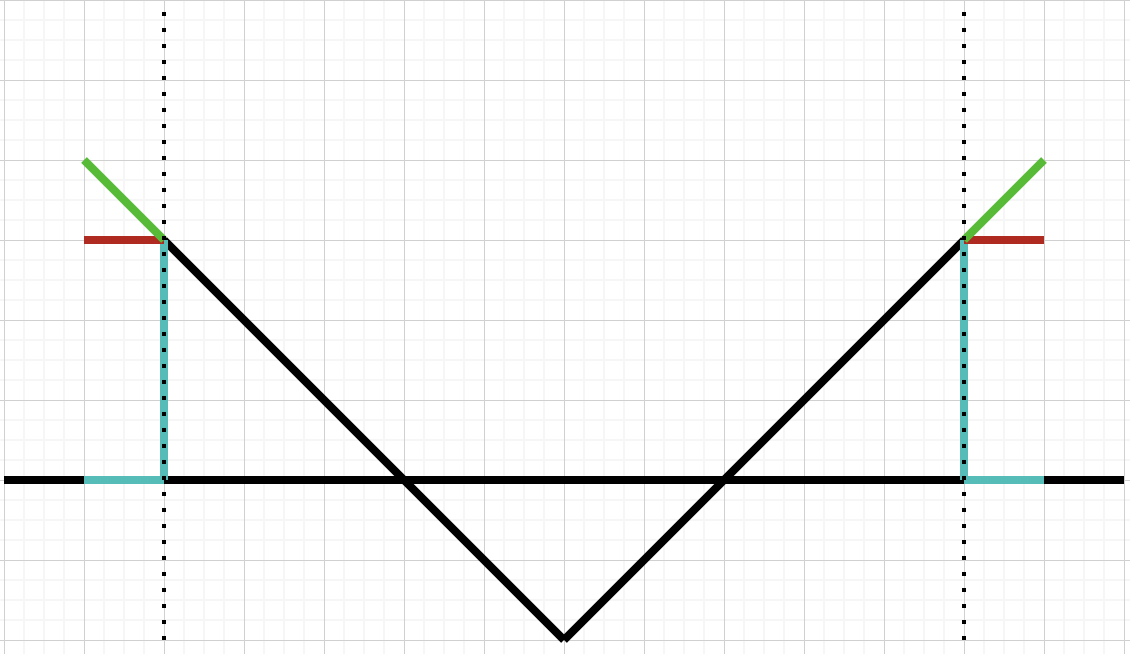
\includegraphics[width=0.51\linewidth]{Materials/MeanFlow/Boundaries}
	\caption{A signed distance field depicted in black along three different choices for padding to handle boundary conditions.}
	\label{boundaryConditions}
\end{figure}
In blue we have a Dirichlet boundary condition where the chosen constant is zero. As we see in \autoref{boundaryConditions} this gives a very abrupt change in the curvature at the boundary. Simply padding our signed distance field from this week's notebook with zeros gives us the following results seen in \autoref{dirichlet}.
\begin{figure}[H]
	\centering
	\begin{subfigure}[b]{0.45\linewidth}
		\centering
		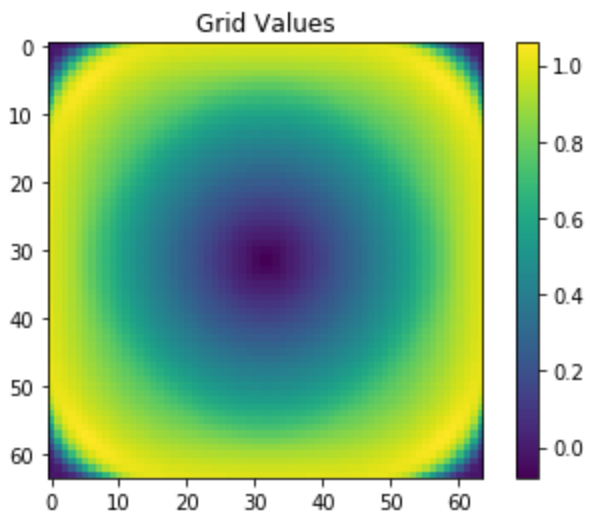
\includegraphics[width=\linewidth]{Materials/MeanFlow/d1}
		\caption{}
		\label{d1}
	\end{subfigure}
	\hfill
	\begin{subfigure}[b]{0.45\linewidth}
		\centering
		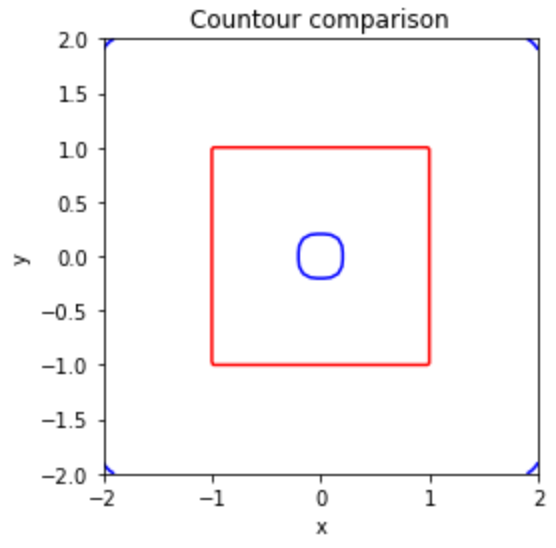
\includegraphics[width=\linewidth]{Materials/MeanFlow/d2}
		\caption{}
		\label{d2}
	\end{subfigure}
	\caption{Padding our signed distance field with zeros before applying mean curvature flow. (A) Image of the grid after applying mean curvature flow. (B) Contours of the grid. Red contours are from before applying mean curvature flow, and blue contours are from after.}
	\label{dirichlet}
\end{figure}
We here note how the corners of the resulting grid have values close to zero but the rest of the grid seems to have increasing values when we move from the center towards the boundaries. In \autoref{d2} we note the slight oval shape of the center blue contour, and how we can see the corner contours.\\
The red boundary condition from \autoref{boundaryConditions} is a von Neumann boundary condition, that is we have $\frac{\partial \phi}{\partial x} = 0$. When discretizing this by using central difference approximations, we find we can implement this by mirroring the values inside the grid along the border to the padded layer. Hence we see in \autoref{boundaryConditions} the red boundary condition stays constant for the last value in the signed distance field. The results of using a von Neumann boundary condition can be seen in \autoref{neumann}.
\begin{figure}[H]
	\centering
	\begin{subfigure}[b]{0.45\linewidth}
		\centering
		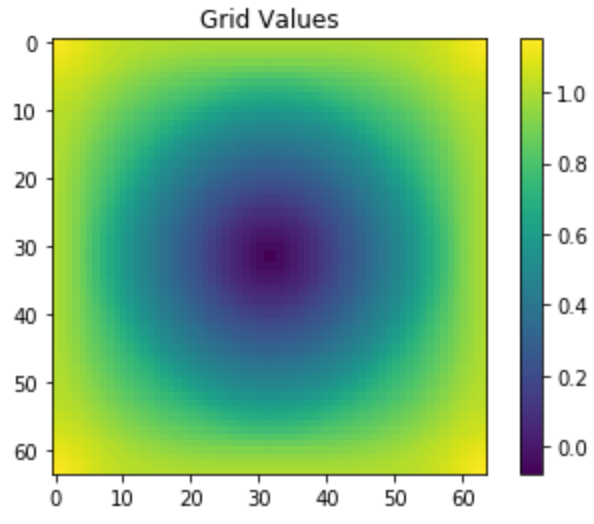
\includegraphics[width=\linewidth]{Materials/MeanFlow/n1}
		\caption{}
		\label{n1}
	\end{subfigure}
	\hfill
	\begin{subfigure}[b]{0.45\linewidth}
		\centering
		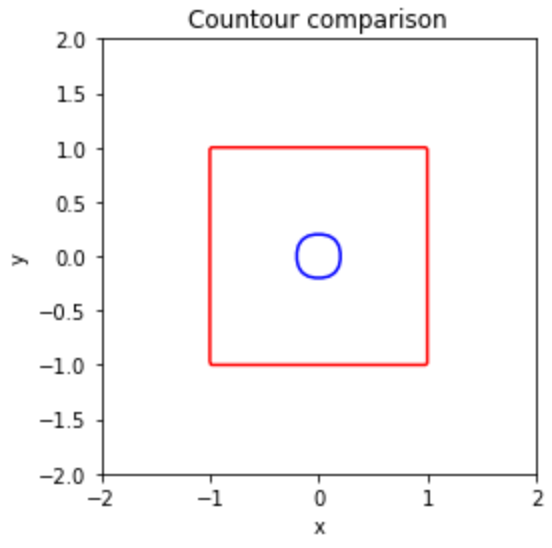
\includegraphics[width=\linewidth]{Materials/MeanFlow/n2}
		\caption{}
		\label{n2}
	\end{subfigure}
	\caption{Padding our signed distance field with mirrored values before applying mean curvature flow. (A) Image of the grid after applying mean curvature flow. (B) Contours of the grid. Red contours are from before applying mean curvature flow, and blue contours are from after.}
	\label{neumann}
\end{figure}
We here note how the values of the grid always increase as we move from the center to the boundaries, and how the blue contour of \autoref{n2} is completely circular and is the only contour after applying the mean curvature flow.\\
The last boundary condition is depicted in green in \autoref{boundaryConditions} and is $\frac{\partial^2 \phi}{\partial x^2} = 0$. As depicted in \autoref{boundaryConditions} this would represent the continuation of the signed distance field as if there were no boundary. I have not been implementing this boundary condition as the discretization of $\frac{\partial^2 \phi}{\partial x^2} = 0$ quickly becomes rather cumbersome. However, this boundary condition will be included in the following discussion of the results.

\subsection{Discussion of results}
A natural question is which boundary condition yields the best results? To answer this, we again look at \autoref{boundaryCondition}. When computing values for our grid we would prefer never to have a boundary, and so naturally using $\frac{\partial \phi}{\partial x} = 0$ as our boundary condition would give us this effect, as this would 'continue our signed distance field'. However, it is cumbersome to implement and a much simpler solution is the von Neumann boundary condition. Although it does not 'continue' the function, it does not make an abrupt change, and when we add together the nodes in the neighbourhood around a boundary node, it does not 'do anything unexpected'. We can compare this to the Dirichlet boundary condition which to some extend could be described as 'removing' the node value. That is, when we add together the neighbourhood we are gonna miss a term which is roughly as big as the value of the boundary node. This is why probably why in our results we see that the corners of the mean curvature flow using Dirichlet boundary conditions are bending downwards whereas the results when using von Neumann are much more 'continuous'. We thus find $\frac{\partial \phi}{\partial x} = 0$ would be the best boundary condition, but because it is hard to implement the von Neumann boundary condition is a good backup.